\subsection{Existing Solutions}

In 1878, Leland Stanford, then Governor of California, commissioned Eadweard Myrbridge to find out whether, when trotting, all four of a horses feet left the ground at the same time \cite{raibert_legged_1986}.
It was proven to be so, and for almost a century, various mechanical designs with fixed moving patterns emerged.
In the 70s, digital computers allowed for on-the-fly kinematic calculations, resulting in more sophisticated mechanical designs and control methods.
In 1984, Dr. Marc Raibert developed a hopping robot with a custom control system, and in 1986 released his seminal piece \textit{Legged Robots that Balance}, covering control methods for robots that are monopedal, bipedal, quadrupedal and beyond.
Since then, the biomimetics scene has exploded, with Dr. Raibert founding Boston Dynamics, arguable the best known company creating the class of robots.
This section of the literature report will detail various existing biomimetic robots from the last decade.

\subsubsection{MiniHyQ}

MiniHyQ is a quadrupedal, hydraulically actuated robot developed by Hamza Khan (see Figure \ref{fig:minihyq_cad}) \cite{khan_development_2015}.
It builds upon the work of various other quadrupedal, hydraulically actuated robots such as Boston Dynamics' Wildcat, Spot and BigDog, MIT Cheetah, and StarIETH, among others.
It was, at the time of publication, the lightest hydraulically actuated quadrupedal robot, weighing 35kg with the on-board hydraulic power pack, in contrast to the similarly sized, 120 kg BigDog \cite{khan_minihyq_2015}.
Its hydraulic system has a maximum power consumption of 5.5 kW.

MiniHyQ has four 3 DOF hydraulically actuated legs; the hip adduction-abduction and knee flexion-extension are powered by Fluitronics AZ013 linear hydraulic actuators, while the hip flexion-extension is powered by an unnamed single-vane rotary hydraulic actuator \cite{khan_minihyq_2015}.
Thanks to a unique 4-bar linkage design, the isometric knee has a changeable center of rotation much like the human knee, providing $180^{\circ}$ of rotation, an improvement on the $120^{\circ}$ range of motion found on the original HyQ and BigDog that limited their mobility and ability to self-right after an incident. It also improves the torque profile, resulting in a smoother motion.

\begin{figure}[H]
    \centering
    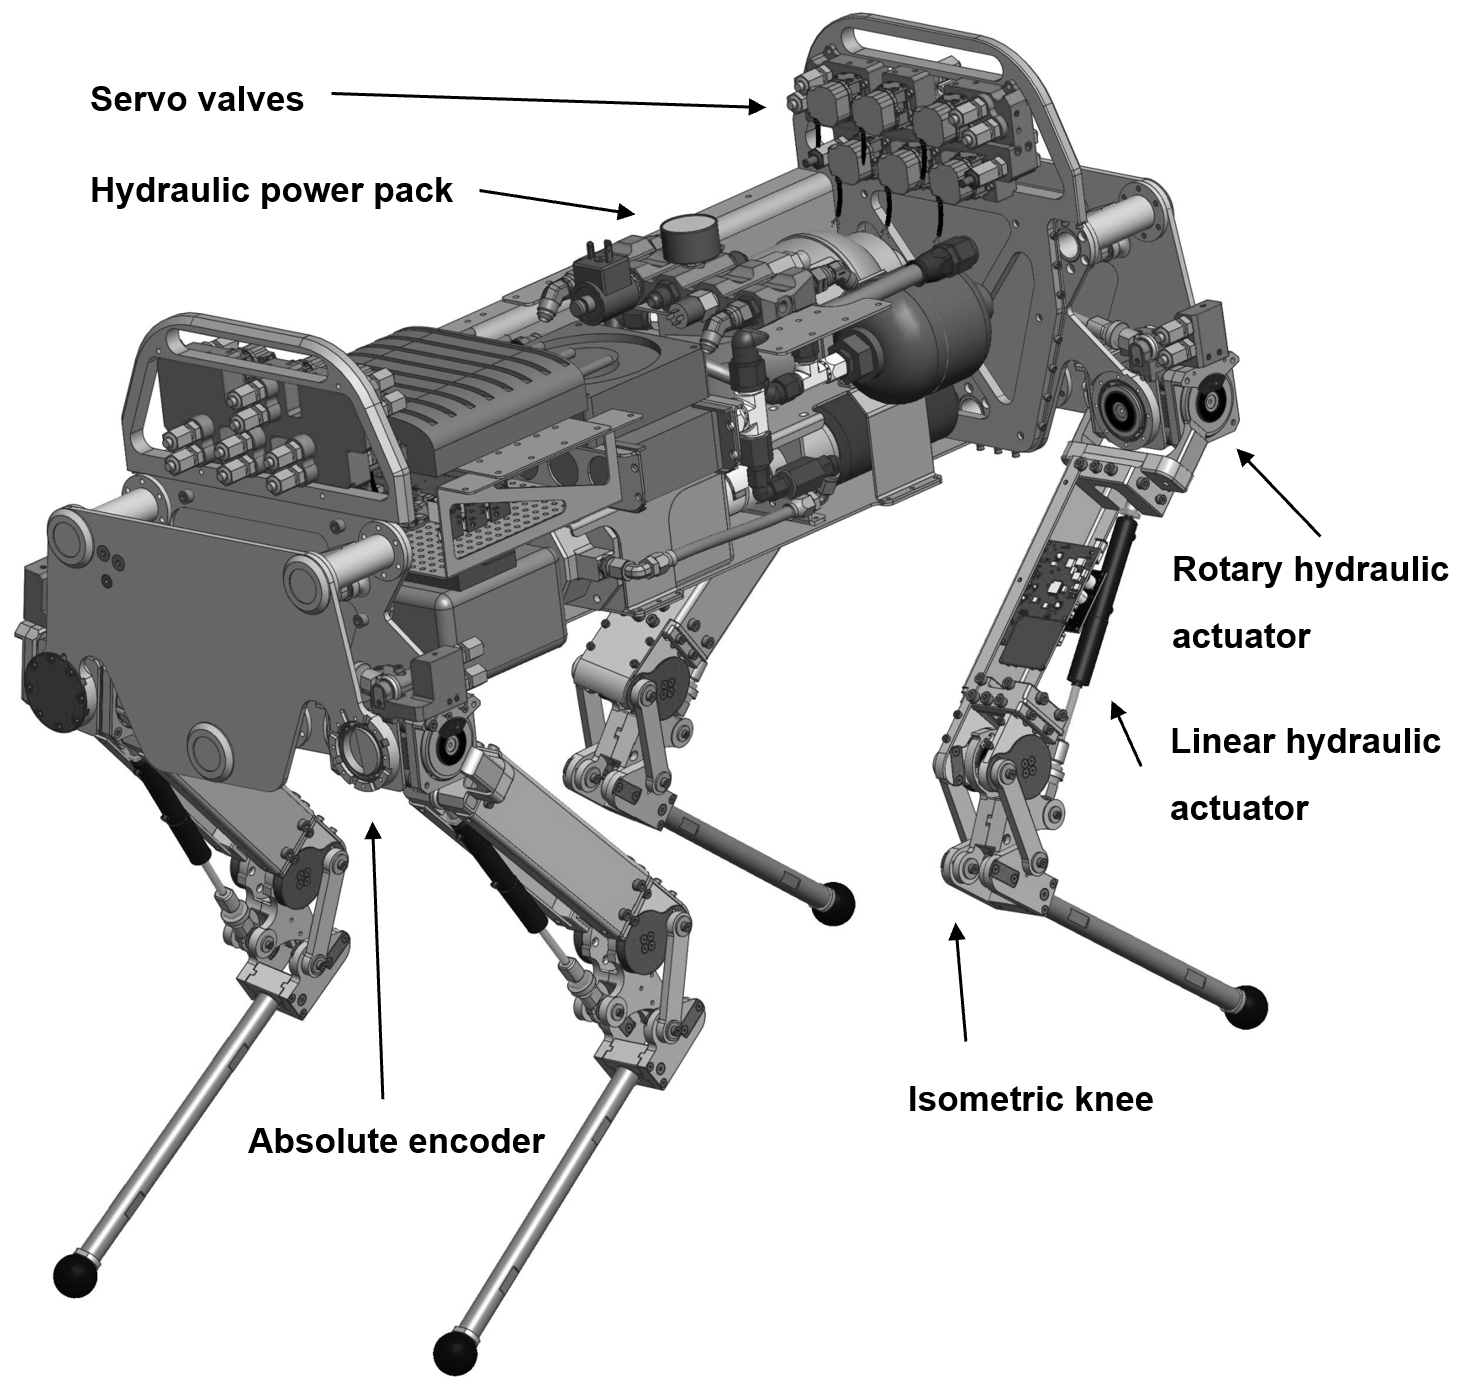
\includegraphics[width=0.8\textwidth]{Sections/LiteratureReview/img/minihyq/exsol_minihyq.png}
    \caption{CAD model of MiniHyQ \cite{khan_minihyq_2015}}
    \label{fig:minihyq_cad}
\end{figure}

\subsubsection{GOAT}

GOAT is an omni-directional leg morphology designed by Simon Kalouche.  It is shown in Figure \ref{fig:goat_img}. It provides a more consistent force profile across the entire leg work-space than traditional series-articulated or redundantly-articulated morphologies. It also provides excellent energy delivery, low limb inertia and high limb acceleration \cite{kalouche_design_2016}.
Each leg's mass budget (ratio of actuator mass to total mass) is 58\%, compared to 40\% and 24\% for Penn Minotaur and MIT Cheetah.

\begin{figure}[H]
    \centering
    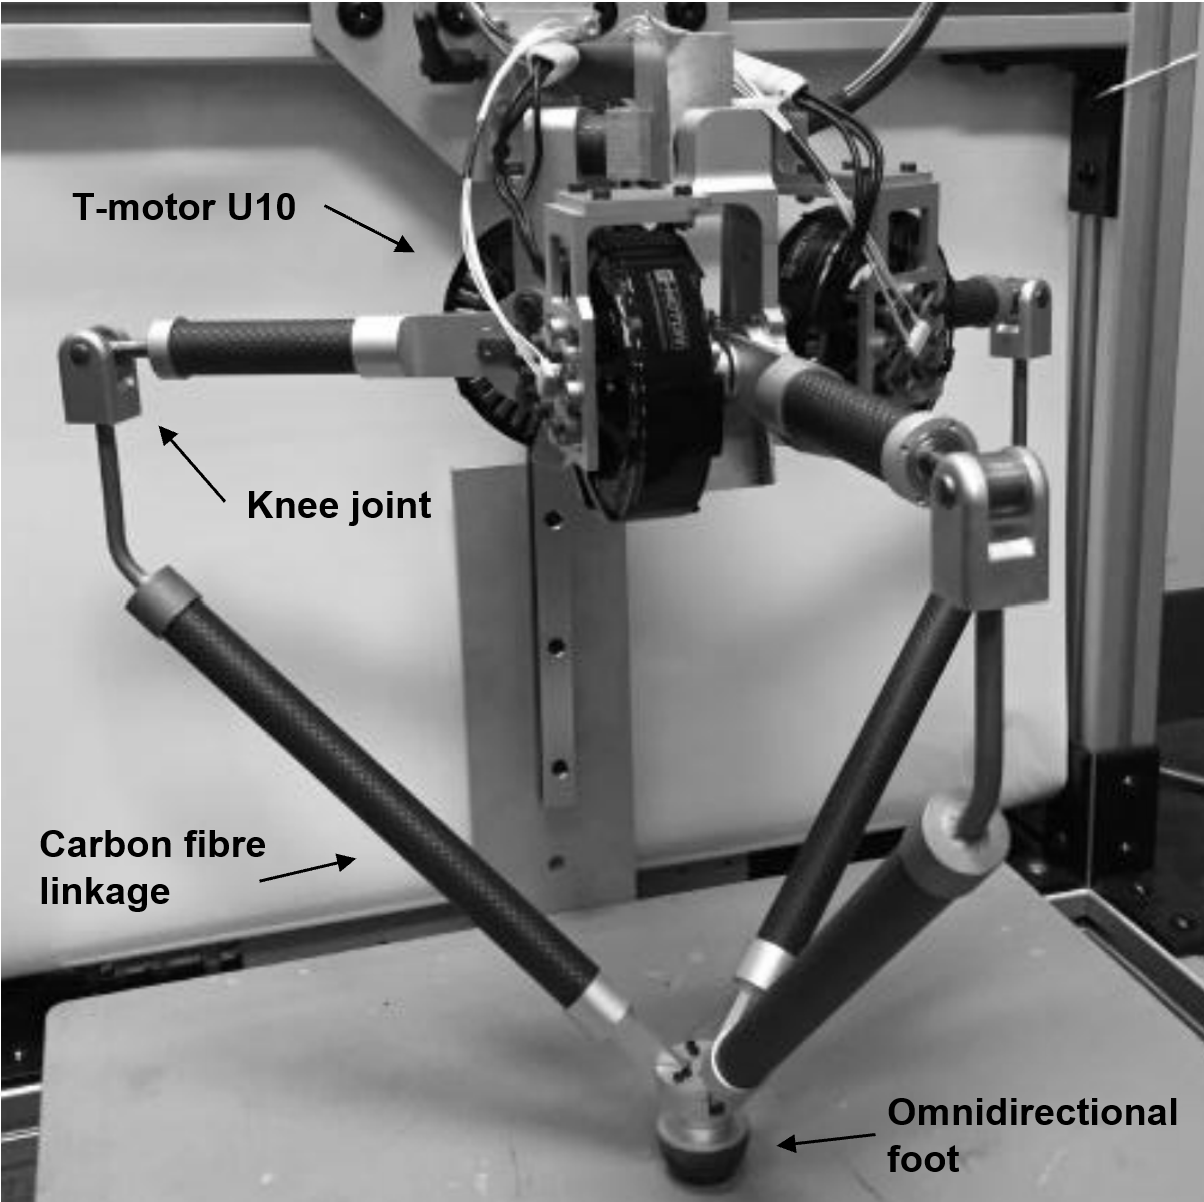
\includegraphics[width=0.8\textwidth]{Sections/LiteratureReview/img/goat/exsol_goat.png}
    \caption{GOAT omni-directional leg \cite{kalouche_design_2016}}
    \label{fig:goat_img}
\end{figure}

\subsubsection{Stanford Doggo}

The Stanford Doggo, as shown in Figure \ref{fig:doggo_img}, is a small quadrupedal robot created by the Stanford Student Robotics team \cite{kau_nate711/stanforddoggoproject_2019}. It is designed to be low cost, lightweight and agile. Its overall price is estimated at around \$3000 and the robot weighs only 4.8 kg. Its leg morphology is made to mimic some of the animals which have the best vertical jumping agility, such as the galago. This is done using a SCARA flavored linkage mechanism with two degrees of freedom (each leg can rotate $360^{\circ}$ and change its height by compression/extension). This allows the Doggo to perform walking, trotting, bounding and pronking. To power the Doggo, two batteries are used which together can provide 44.4 Wh of energy. The maximum continuous power consumption is 840 W \cite{kau_stanford_2019}. The controller system consists of one micro-controller that calculates leg trajectories and sends commands to four ODrive motor controllers (one for each leg). Power is distributed from the battery to the various electric components via a power distribution board \cite{kau_stanford_2019}. 

\begin{figure}[H]
    \centering
    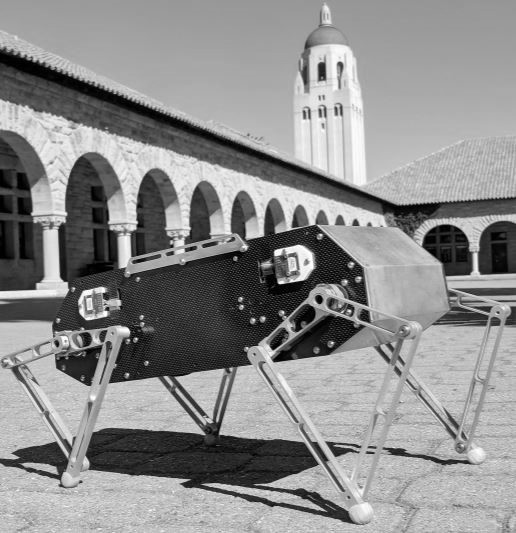
\includegraphics[width=0.7\textwidth]{Sections/LiteratureReview/img/doggo/exsol_doggo.JPG}
    \caption{Stanford Doggo quadrupedal robot \cite{kau_stanford_2019}}
    \label{fig:doggo_img}
\end{figure}

\subsubsection{Machining Hexapod}

Murschiduzzaman et al developed a small hexapod robot, shown in Figure \ref{fig:cnchexopod_cad} \cite{murshiduzzaman_hexapod_2019}, to act as a portable CNC machine, reducing the need for large, permanent equipment \cite{murshiduzzaman_hexapod_2019}. Its six-legged design provides additional mechanical stability, compared to the previous quadrupedal robots which rely more heavily on state-of-the-art controls to maintain their stability \cite{bottcher_principles_nodate}. 
System weight and power were not provided by the author.

\begin{figure}[H]
    \centering
    \includegraphics[width=0.8\textwidth]{Sections/LiteratureReview/img/cnchexopod/exsol_cnchexapod.png}
    \caption{Hexapod robot; note the spindle attached for CNC-ing small parts \cite{murshiduzzaman_hexapod_2019}}
    \label{fig:cnchexopod_cad}
\end{figure}

\subsubsection{Hexapod v2.1}

Hexapod v2.1 is a small hexapod robot designed and built as a personal hobby project by an internet user named Smallp Tsai \cite{smallp_tsai_hexapod_2018}. The hexapod illustrated in Figure \ref{fig:hexapodv2p1_img} consists of six 3D printed legs and a chassis. It uses the tripod gait which provides constant stability on rough terrains. Each leg is driven by three MG92B servo motors that are controlled by a set of PCBs and powered by a 7.4 V battery. Each servo motor can produce a stall torque of 3.5 kg/cm and an operating speed of $\frac{60^{\circ}}{0.08\texttt{ sec}}$ when powered with 6 V \cite{tower_pro_mg92b_nodate}. It is capable of moving forward in a linear or curvilinear motion. The hexapod has also a climb mode which slightly elevates its body and increases the vertical displacement of each leg when going up a slope.

\begin{figure}[H]
    \centering
    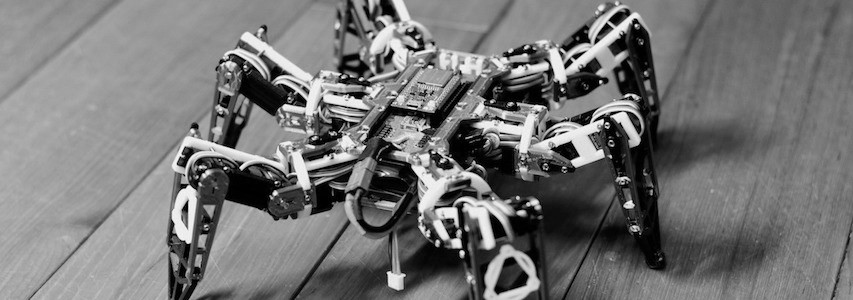
\includegraphics[width=0.8\textwidth]{Sections/LiteratureReview/img/hexapodV2.1/hexapod_v2p1.jpg}
    \caption{Hexapod v2.1 \cite{smallp_tsai_hexapod_2018}}
    \label{fig:hexapodv2p1_img}
\end{figure}

\subsubsection{CRABSTER200}

CRABSTER200 (CR200) is a large hexapod robot designed by the Korean Institute of Ocean Science and Technology (KIOST) \cite{shim_development_2016}. Its main purpose is to conduct seabed mapping and other surveying activities on the seabed at a depth of approximately 200 m. Each joint of the 4 DOF legs includes a motor, giving a subtotal of 24 motors dedicated to the locomotion of the hexapod. Nitrile rubber type O-rings and dual O-rings are used to offer a watertight housing for each joint. CR200 is also equipped with a gripper in each of its front legs, and houses other devices in its hull such as cameras, sensors, and communicating equipment, as shown in Figure \ref{fig:crabsterdetailed_img}.

\begin{figure}[H]
    \centering
    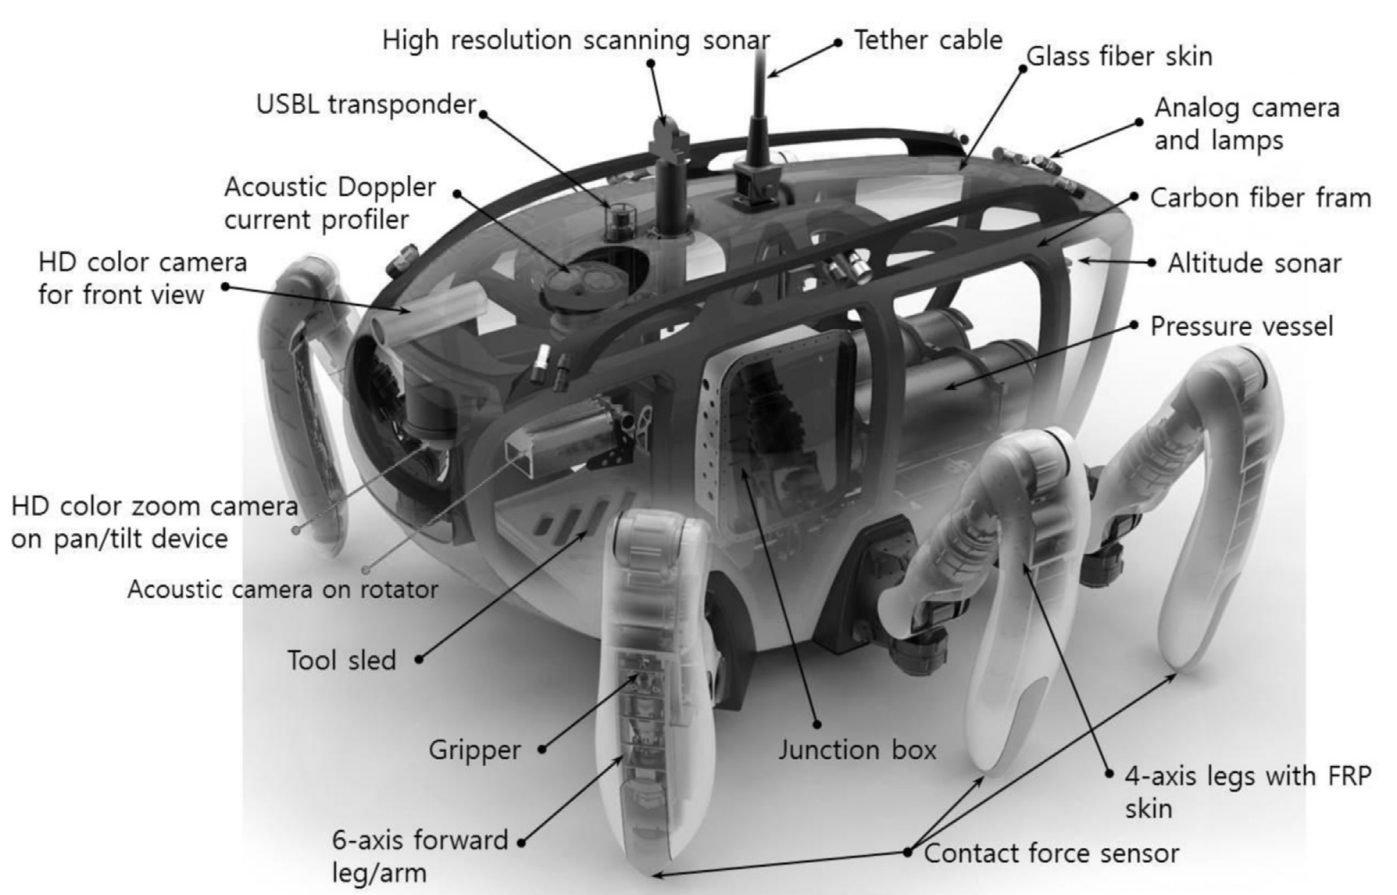
\includegraphics[width=0.8\textwidth]{Sections/LiteratureReview/img/Crabster/crabster_detailed.jpg}
    \caption{Concept of multi-legged seabed walking robot (CR200) \cite{shim_development_2016}}
    \label{fig:crabsterdetailed_img}
\end{figure}